\documentclass[journal=jcisd8,manuscript=article]{achemso}

\usepackage{hyperref}
\usepackage{graphicx}
\usepackage{longtable}
\usepackage{subfig}
\usepackage{array}

\graphicspath{ {./resources/} }
\newcolumntype{P}[1]{>{\centering\arraybackslash}p{#1}}

\newcommand*\mycommand[1]{\texttt{\emph{#1}}}
\renewcommand{\thefootnote}{\fnsymbol{footnote}}

\author{Vineeth Chelur}
\author{U. Deva Priyakumar}
\email{deva@iiit.ac.in}
\affiliation[IIIT-H]
{Center for Computational Natural Sciences \& Bioinformatics \\ International Institute of Information Technology \\ Hyderabad - 500032, India}

\title[BiRDS - Binding Residue Detection from Protein Sequences using Deep ResNets. Supporting Information.]
  {BiRDS - Binding Residue Detection from Protein Sequences using Deep ResNets. Supporting Information.}

\begin{document}

\thispagestyle{empty}

\tableofcontents

\listoftables

\listoffigures

\pagenumbering{arabic}

\newpage

\addcontentsline{toc}{section}{Evaluation Metrics}
\section{Evaluation Metrics}
\subsection{Confusion Matrix}
A confusion matrix is a table that allows for the visualisation of the performance of a supervised learning algorithm. The following terminologies can be defined in the binary classification of a residue as a binding residue (BR) or non-binding residue (NBR).
\begin{itemize}
    \item True Positive (TP): Number of BRs predicted correctly as BRs.
    \item True Negative (TN): Number of NBRs predicted correctly as NBRs.
    \item False Positive (FP): Number of NBRs predicted incorrectly as BRs.
    \item False Negative (FN): Number of BRs predicted incorrectly as NBRs.
\end{itemize}

\noindent The following metrics can be derived from the confusion matrix

Accuracy: ${ACC} = \frac{TP + TN}{TP + TN + FP + FN}$

Precision: ${PPV} = \frac{TP}{TP + FP}$

Recall: ${TPR} = \frac{TP}{TP + FN}$

F1 score: ${F_1} = \frac{2TP}{2TP + FP + FN}$

Matthews Correlation Coefficient: ${MCC} = \frac{TP \times TN - FP \times FN}{\sqrt{(TP + FP)(TP + FN)(TN + FP)(TN + FN)}}$

\subsection{MCC}
\quad The Matthew's Correlation varies from $[-1, +1]$, with $+1$ representing a perfect prediction, 0 representing no better than a random prediction and -1 representing total disagreement between the prediction and the observation.


% Different Resnet basic block input and output sizes, $d$ and $e$, were tested, but the values shared in the architecture were the most optimal in terms of faster training time and better metrics. Increasing/Decreasing the filter size of the convolutional layers either worsened the performance or lengthened the training time of the model with no additional benefit.


% TODO: Update the below table and insert it here
% \begin{table}
%   \centering
%   \begin{tabular}{| P{2.75cm} | P{2.75cm} | P{2.75cm} | P{2.75cm} | P{2.75cm} |}
%       \hline
%             & $N_{prot}$ & $N_{br}$ & $N_{nbr}$ & $P_{br}(\%)$ \\
%       \hline
%       Train & 16,450     & 589,329  & 8,725,043 & 6.33         \\
%       % Valid & 1586       &          &           &              \\
%       Test  & 2,464      & 86,230   & 1,345,646 & 6.02         \\
%       \hline
%   \end{tabular}
%   \caption{\label{tab:dataset_summary} Summary of the dataset used for training and testing}
%   \vspace{5 mm}
%   \noindent $N_{prot}$ - Number of proteins \hfill $N_{br}$ - Total number of binding residues

%   \vspace{3 mm}

%   \noindent $N_{nbr}$ - Total number of non-binding residues \hfill $P_{br}(\%)$ - Percentage of binding residues
% \end{table}

% \newpage
% \begin{center}
%   \begin{longtable}{|l|l|l|}
%     \caption{Train Set - Sequences with no MSA hits}
%     \label{table:trainsinglemsa}                                                                                                                  \\

%     \hline \multicolumn{1}{|c|}{\textbf{First column}} & \multicolumn{1}{c|}{\textbf{Second column}} & \multicolumn{1}{c|}{\textbf{Third column}} \\ \hline
%     \endfirsthead

%     \multicolumn{3}{c}%
%     {{\bfseries \tablename\ \thetable{} -- continued from previous page}}                                                                         \\
%     \hline \multicolumn{1}{|c|}{\textbf{First column}} & \multicolumn{1}{c|}{\textbf{Second column}} & \multicolumn{1}{c|}{\textbf{Third column}} \\ \hline
%     \endhead

%     \hline \multicolumn{3}{|r|}{{Continued on next page}}                                                                                         \\ \hline
%     \endfoot

%     \hline \hline
%     \endlastfoot

%     1a4w                                               & I                                           & NGDFEEIPEEYL                               \\
%     1ae8                                               & I                                           & DFEEIPEEYL                                 \\
%     1bc5                                               & T                                           & XNWETF                                     \\
%     1c4u                                               & 3                                           & ACENEDFEGIPGEY                             \\
%     1c4v                                               & 3                                           & ACENEDFEEIPGEYL                            \\
%     1c4y                                               & 3                                           & ENEDFEGIPGEYL                              \\
%     1g5q                                               & M                                           & DSYTC                                      \\
%     1gul                                               & M                                           & EXG                                        \\
%     1gwq                                               & C                                           & KILHRLLQD                                  \\
%     1gwr                                               & C                                           & NALLRYLLD                                  \\
%     1gy3                                               & E                                           & HHASPRK                                    \\
%     1nq7                                               & B                                           & HKILHRLLQE                                 \\
%     1nt1                                               & H                                           & DFEEIPEAYLA                                \\
%     1nvq                                               & B                                           & ASVSA                                      \\
%     1nzq                                               & D                                           & XYEPIPEEFAQ                                \\
%     1o6k                                               & C                                           & GRPRTTSFAE                                 \\
%     1orh                                               & B                                           & GGFGGRGGFG                                 \\
%     1osv                                               & C                                           & ENALLRYLLDKD                               \\
%     1oyt                                               & I                                           & XFEEIPEEYLQ                                \\
%     1p93                                               & E                                           & KENALLRYLLDK                               \\
%     1piv                                               & 0                                           & ISEV                                       \\
%     1pn3                                               & C                                           & XXNGGXX                                    \\
%     1qbq                                               & P                                           & XCVIM                                      \\
%     1qsn                                               & B                                           & KSTGGKAPRKQ                                \\
%     1sb1                                               & I                                           & DFEEIPEEY                                  \\
%     1soz                                               & D                                           & DNRLGLVYQF                                 \\
%     1t5z                                               & B                                           & RETSEKFKLLFQSYN                            \\
%     1t73                                               & B                                           & SRFADFFRNEGLGSRSGSGK                       \\
%     1t74                                               & B                                           & SRWQALFDDGTDTSR                            \\
%     1t76                                               & B                                           & SRWAEVWDDNSKVSR                            \\
%     1t79                                               & B                                           & SSKFAALWDPPKLSRSGSGK                       \\
%     1t7f                                               & B                                           & SSRGLLWDLLTKDSRSGSGK                       \\
%     1t7m                                               & B                                           & SSNTPRFKEYFMQSRSGSGK                       \\
%     1t7r                                               & B                                           & SSRFESLFAGEKESR                            \\
%     1u3r                                               & C                                           & SGSHKLVQLLTTT                              \\
%     1u9e                                               & C                                           & KLVQLLTTT                                  \\
%     1uhl                                               & C                                           & HKILHRLLQD                                 \\
%     1w7g                                               & I                                           & NEDFEEIPEEYL                               \\
%     1wbp                                               & B                                           & RRRERSPTR                                  \\
%     1x27                                               & J                                           & MEDYDYVHL                                  \\
%     1xb0                                               & G                                           & AVPIAQK                                    \\
%     1xj7                                               & B                                           & HKKLLQLLT                                  \\
%     1xow                                               & B                                           & RGAFQNLFQSV                                \\
%     1y3a                                               & E                                           & SRVTWYDFLMEDTKSR                           \\
%     2a3i                                               & B                                           & QQKSLLQQLLTE                               \\
%     2b9j                                               & C                                           & SKRGNIPKPLNLS                              \\
%     2bil                                               & A                                           & ARKRRRHPSGPPTA                             \\
%     2bj4                                               & C                                           & LTSRDFGSWYA                                \\
%     2bxt                                               & I                                           & GDFEEIPEEYL                                \\
%     2c3i                                               & A                                           & KRRRHPSG                                   \\
%     2cch                                               & E                                           & HTLKGRRLVFDN                               \\
%     2cvy                                               & B                                           & GAFTFNEDF                                  \\
%     2fvj                                               & B                                           & QTSHKLVQLLTTT                              \\
%     2g2f                                               & C                                           & EAIFAAPFAKK                                \\
%     2gde                                               & D                                           & DFEEIPGEYL                                 \\
%     2ght                                               & D                                           & SYSPTSPS                                   \\
%     2gtk                                               & B                                           & HKLVQLLTTT                                 \\
%     2h96                                               & F                                           & RPKRPTTLNLF                                \\
%     2hu2                                               & B                                           & RRTGAPPAL                                  \\
%     2jam                                               & D                                           & GVSKFA                                     \\
%     2jam                                               & E                                           & VSKF                                       \\
%     2jf9                                               & P                                           & SPGSREWFKDMLS                              \\
%     2oy2                                               & Y                                           & IAG                                        \\
%     2p0r                                               & D                                           & XLLR                                       \\
%     2p54                                               & B                                           & ARHKILHRLLQE                               \\
%     2pkl                                               & B                                           & KLLF                                       \\
%     2q5y                                               & D                                           & SKYGLQD                                    \\
%     2qll                                               & B                                           & GPYY                                       \\
%     2qpy                                               & B                                           & LLRYLLDKDD                                 \\
%     2qt5                                               & Y                                           & NNLQDGTEV                                  \\
%     2r3y                                               & E                                           & DNRLGLVYWF                                 \\
%     2x1n                                               & H                                           & XLNFX                                      \\
%     2x72                                               & B                                           & ILENLKDCGLF                                \\
%     3m53                                               & B                                           & XSKSKDRKYTL                                \\
%     3swc                                               & P                                           & SATARKVGRPGR                               \\
%     3vri                                               & C                                           & RVAQLEQVYI                                 \\
%     3zg6                                               & F                                           & KQTARXSTGGWW                               \\
%     4au7                                               & C                                           & RHRKVLRDY                                  \\
%     4nie                                               & D                                           & KHKILHRLLQDS                               \\
%     5ax3                                               & B                                           & LVKKYILALWNE                               \\
%     5cxv                                               & C                                           & DYKDDDD                                    \\
%     5ex0                                               & D                                           & EKFGKGGTYP                                 \\
%     \hline
%   \end{longtable}
% \end{center}

\begin{center}
    \begin{table}[ht]
        \centering
        \begin{tabular}{|c|c|}
            \hline
            \textbf{Obsoleted PDB IDs} & \textbf{Replacement PDB IDs} \\
            \hline
            1HWZ                       & 6DHD                         \\
            1QY5                       & 6D28                         \\
            1U0Y                       & 6D1X                         \\
            2CMJ                       & 5YZH                         \\
            2CMV                       & 5YZI                         \\
            2PDT                       & 6CNY                         \\
            3G07                       & 5UNA                         \\
            3KWN                       & 5QC4                         \\
            3LNS                       & 3LNS                         \\
            3LV1                       & 3LV1                         \\
            3MPE                       & 5QBY                         \\
            3MVQ                       & 6DHL                         \\
            3MW9                       & 6DHM                         \\
            3N3N                       & 5SXQ                         \\
            3Q9K                       & 6L9E                         \\
            3QL6                       & 6LAQ                         \\
            3TUW                       & 5ZGS                         \\
            4DGO                       & 6QS5                         \\
            4EGB                       & 6BI4                         \\
            4GDC                       & 5VWT                         \\
            4GDD                       & 5VWU                         \\
            4KA6                       & 5SYI                         \\
            4KG1                       & 5H5O                         \\
            4KNZ                       & 6NNR                         \\
            4N3L                       & 6EO8                         \\
            4N7A                       & 6LF7                         \\
            4NT3                       & 6LCO                         \\
            4NZE                       & 6EO9                         \\
            4OA9                       & 5LPV                         \\
            4OAC                       & 5LPB                         \\
            4OTW                       & 6OP9                         \\
            4P7P                       & 5I0K                         \\
            4PT0                       & 5GTK                         \\
            4PT3                       & 5GTL                         \\
            4UTD                       & 6CPF                         \\
            4WBN                       & 6I5C                         \\
            4Y9Q                       & 5MF5                         \\
            5AAJ                       & 5OMO                         \\
            5CTO                       & 6J63                         \\
            5LI5                       & 5LX2                         \\
            \hline
        \end{tabular}
        \caption{Train Set - Obsoleted PDB IDs along with replacement PDB IDs}
        \label{table:trainobsoleted}
    \end{table}
\end{center}
\clearpage

\begin{center}
    \begin{table}[ht]
        \centering
        \begin{tabular}{|c c c c c|}
            \hline
            5MWR & 5X8O & 6C2L & 6ELH & 6I2L \\
            5MYH & 5YV4 & 6C2P & 6EMC & 6IQ7 \\
            5MZ9 & 5Z3T & 6C38 & 6EME & 6IQ8 \\
            5N7R & 5Z4I & 6CB4 & 6ESO & 6IRM \\
            5NWO & 5ZBV & 6CO0 & 6ETX & 6IRN \\
            5OLI & 5ZD5 & 6CSY & 6FJR & 6JLW \\
            5UF9 & 5ZD7 & 6CU4 & 6FMM & 6JLX \\
            5UUR & 6A5V & 6D4J & 6FO4 & 6JU2 \\
            5VB1 & 6ABB & 6D5I & 6FOT & 6JU3 \\
            5VB4 & 6ABD & 6DM2 & 6FOU & 6MPU \\
            5VFL & 6ABE & 6DTJ & 6FOV & 6MSZ \\
            5VG5 & 6ABF & 6DU1 & 6FPE & 6N3T \\
            5WVQ & 6ABG & 6DUA & 6FQC & 6NLC \\
            5WVS & 6BW7 & 6DX6 & 6G9Y & 6NLD \\
            5WVT & 6C0C & 6E5O & 6GJX & 6NPG \\
            5WW1 & 6C2E & 6E79 & 6GKP & 6NXH \\
            5WW2 & 6C2J & 6E7A & 6H7K & 6UHD \\
            5WWA & 6C2K & 6EDO & 6HBO &      \\
            \hline
        \end{tabular}
        \caption{Test Set Removed - Obsoleted PDBs}
        \label{table:testobsoleted}
    \end{table}
\end{center}
\clearpage

\begin{center}
    \begin{table}[ht]
        \centering
        \begin{tabular}{|c|}
            \hline
            6DC9 \\
            6DCA \\
            6EOD \\
            6FE0 \\
            6FE1 \\
            6IEY \\
            6MQC \\
            6MQE \\
            6N16 \\
            6NCP \\
            6RUL \\
            6SNC \\
            6SND \\
            6SNE \\
            \hline
        \end{tabular}
        \caption{Test Set Removed - Reindexing Errors}
        \label{table:testreindex}
    \end{table}
\end{center}
\clearpage

\begin{figure}[h]%
    \centering
    \subfloat[\centering No PSSM and IC features]{{ \label{fig:no_pssm_cm} 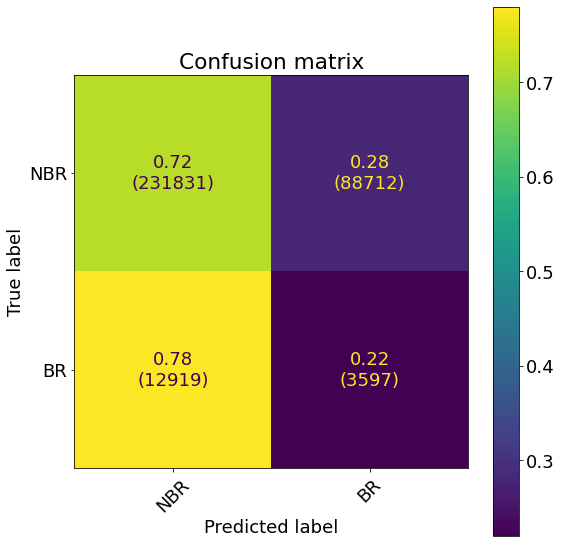
\includegraphics[width=0.45\textwidth]{no_pssm_cm.png} }}
    \qquad
    \subfloat[\centering No Embedding features]{{ \label{fig:no_embeddings_cm} 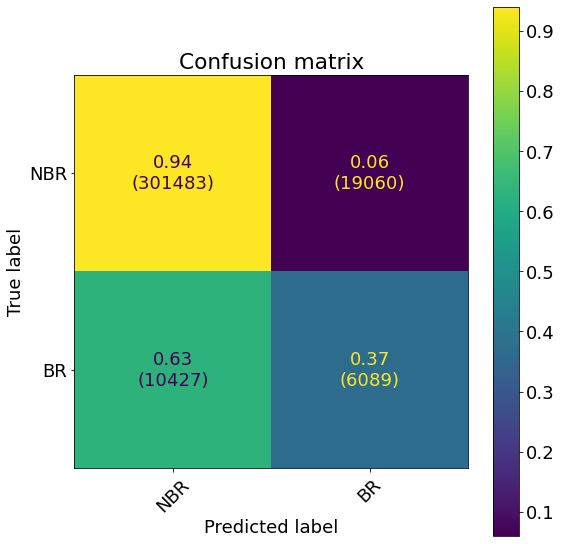
\includegraphics[width=0.45\textwidth]{no_embeddings_cm.png} }}
    \subfloat[\centering No SS3 and RSA features]{{ \label{fig:no_ss3_rsa_cm} 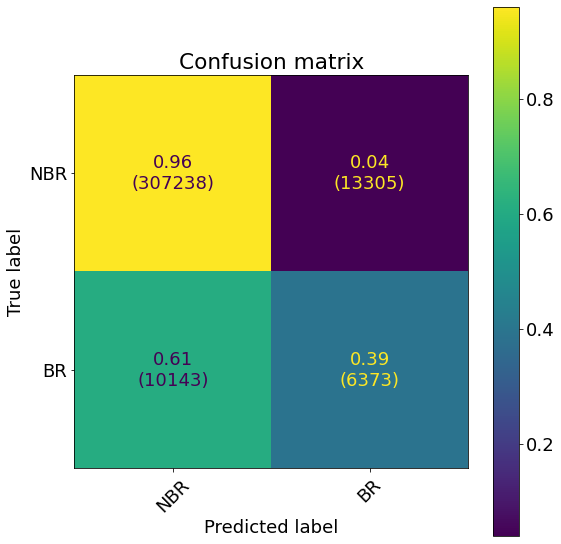
\includegraphics[width=0.45\textwidth]{no_ss3_rsa_cm.png} }}
    \vspace{1em}
    \caption{\centering Confusion matrix of the Ablation Study on the reduced test set}%
    \label{fig:test_cm}%
\end{figure}


% \begin{center}
%   \begin{table}[ht]
%     \centering
%     \begin{tabular}{|c|}
%       \hline
%       6EQO \\
%       5WMM \\
%       5O9U \\
%       5O9V \\
%       5Y2D \\
%       6EJ7 \\
%       6MM5 \\
%       6EXN \\
%       6FF4 \\
%       6KZO \\
%       6KZP \\
%       6OR5 \\
%       6RLA \\
%       6S8F \\
%       6SKY \\
%       6SKZ \\
%       6SL1 \\
%       6U5T \\
%       6U5U \\
%       \hline
%     \end{tabular}
%     \caption{Test Set Removed - Could not generate residue contacts}
%     \label{table:testothers}
%   \end{table}
% \end{center}

% \caption{List of obsoleted PDB IDs in the test set}

% \begin{center}
%     \begin{table}[ht]
%     \centering
%         \begin{tabular}{ccc}
%             \hline
%             \textbf{Fold} & \textbf{Top-n} & \textbf{Top-(n+2)} \\
%             \hline
%             1 & 76.38\% & 91.17\% \\
%             2 & 68.31\% & 89.59\% \\
%             3 & 69.20\% & 86.74\% \\
%             4 & 69.46\% & 85.21\% \\
%             5 & 71.82\% & 89.40\% \\
%             6 & 72.24\% & 89.39\% \\
%             7 & 69.24\% & 89.06\% \\
%             8 & 73.1\% & 89.48\% \\
%             9 & 64.84\% & 82.19\% \\
%             10 & 68.36\% & 85.66\% \\
%             \hline
%             All & 70.27\% & 87.77\% \\
%             \hline
%         \end{tabular}
%         \caption{Top-n and Top-(n+2) success rates of the 10 classification models on their corresponding validation sets}
%         \label{table:supplclassification2}
%     \end{table}
% \end{center}

% \begin{figure}
%     \caption{Test curves of the 10 classification models on their corresponding validation sets during 10-fold cross validation reporting (a) Accuracy, (b) Area under the curve - Receiver operating characteristic (AUC-ROC).}
%     \label{fig:Classification_cross_val_SI}
%     \centering
%     \begin{subfigure}[b]{\textwidth}
%         \begin{subfigure}[b]{0.485\textwidth}
%             \centering
%             \includegraphics[width=\textwidth]{figures/suppl/fold1_acc.png}
%         \end{subfigure}
%         \hfill
%         \begin{subfigure}[b]{0.485\textwidth}
%             \centering
%             \includegraphics[width=\textwidth]{figures/suppl/fold1_auc.png}
%         \end{subfigure}
%         \caption{Fold 1}
%         \label{fig:fold1}
%     \end{subfigure}
%     \hfill
%     \begin{subfigure}[b]{\textwidth}
%         \begin{subfigure}[b]{0.485\textwidth}
%             \centering
%             \includegraphics[width=\textwidth]{figures/suppl/fold2_acc.png}
%         \end{subfigure}
%         \hfill
%         \begin{subfigure}[b]{0.485\textwidth}
%             \centering
%             \includegraphics[width=\textwidth]{figures/suppl/fold2_auc.png}
%         \end{subfigure}
%         \hfill
%         \caption{Fold 2}
%         \label{fig:fold2}
%     \end{subfigure}
%     \begin{subfigure}[b]{\textwidth}
%         \begin{subfigure}[b]{0.485\textwidth}
%             \centering
%             \includegraphics[width=\textwidth]{figures/suppl/fold3_acc.png}
%         \end{subfigure}
%         \hfill
%         \begin{subfigure}[b]{0.485\textwidth}
%             \centering
%             \includegraphics[width=\textwidth]{figures/suppl/fold3_auc.png}
%         \end{subfigure}
%         \caption{Fold 3}
%         \label{fig:fold3}
%     \end{subfigure}
%     \hfill
%     \begin{subfigure}[b]{\textwidth}
%         \begin{subfigure}[b]{0.485\textwidth}
%             \centering
%             \includegraphics[width=\textwidth]{figures/suppl/fold4_acc.png}
%         \end{subfigure}
%         \hfill
%         \begin{subfigure}[b]{0.485\textwidth}
%             \centering
%             \includegraphics[width=\textwidth]{figures/suppl/fold4_auc.png}
%         \end{subfigure}
%         \caption{Fold 4}
%         \label{fig:fold4}
%     \end{subfigure}
% \end{figure}

% \begin{figure}\ContinuedFloat
%      \begin{subfigure}[b]{\textwidth}
%      \begin{subfigure}[b]{0.485\textwidth}
%          \centering
%          \includegraphics[width=\textwidth]{figures/suppl/fold5_acc.png}
%      \end{subfigure}
%      \hfill
%      \begin{subfigure}[b]{0.485\textwidth}
%          \centering
%          \includegraphics[width=\textwidth]{figures/suppl/fold5_auc.png}
%      \end{subfigure}
%      \caption{Fold 5}
%      \label{fig:fold5}
%      \end{subfigure}
%      \hfill
%      \begin{subfigure}[b]{\textwidth}
%      \begin{subfigure}[b]{0.485\textwidth}
%          \centering
%          \includegraphics[width=\textwidth]{figures/suppl/fold6_acc.png}
%      \end{subfigure}
%      \hfill
%      \begin{subfigure}[b]{0.485\textwidth}
%          \centering
%          \includegraphics[width=\textwidth]{figures/suppl/fold6_auc.png}
%      \end{subfigure}
%      \caption{Fold 6}
%      \label{fig:fold6}
%      \end{subfigure}
%      \hfill
%      \begin{subfigure}[b]{\textwidth}
%      \begin{subfigure}[b]{0.485\textwidth}
%          \centering
%          \includegraphics[width=\textwidth]{figures/suppl/fold7_acc.png}
%      \end{subfigure}
%      \hfill
%      \begin{subfigure}[b]{0.485\textwidth}
%          \centering
%          \includegraphics[width=\textwidth]{figures/suppl/fold7_auc.png}
%      \end{subfigure}
%      \caption{Fold 7}
%      \label{fig:fold7}
%      \end{subfigure} 
%      \hfill
%      \begin{subfigure}[b]{\textwidth}
%      \begin{subfigure}[b]{0.485\textwidth}
%          \centering
%          \includegraphics[width=\textwidth]{figures/suppl/fold8_acc.png}
%      \end{subfigure}
%      \hfill
%      \begin{subfigure}[b]{0.485\textwidth}
%          \centering
%          \includegraphics[width=\textwidth]{figures/suppl/fold8_auc.png}
%      \end{subfigure}
%      \caption{Fold 8}
%      \label{fig:fold8}
%      \end{subfigure}
%      \hfill
% \end{figure}
% \begin{figure}[H]\ContinuedFloat
%     \begin{subfigure}{\textwidth}
%      \begin{subfigure}{0.485\textwidth}
%          \centering
%          \includegraphics[width=\textwidth]{figures/suppl/fold9_acc.png}
%      \end{subfigure}
%      \hfill
%      \begin{subfigure}{0.485\textwidth}
%          \centering
%          \includegraphics[width=\textwidth]{figures/suppl/fold9_auc.png}
%      \end{subfigure}
%      \caption{Fold 9}
%      \label{fig:fold9}
%      \end{subfigure}
%      \hfill
%      \begin{subfigure}{\textwidth}
%      \begin{subfigure}{0.485\textwidth}
%          \centering
%          \includegraphics[width=\textwidth]{figures/suppl/fold10_acc.png}
%      \end{subfigure}
%      \hfill
%      \begin{subfigure}{0.485\textwidth}
%          \centering
%          \includegraphics[width=\textwidth]{figures/suppl/fold10_auc.png}
%      \end{subfigure}
%      \caption{Fold 10}
%      \label{fig:fold10}
%      \end{subfigure}
%      \hfill
% \end{figure}

% \clearpage
% \newpage

% \begin{center}
%     \begin{table}[ht]
%     \centering
%         \begin{tabular}{ccc}
%             \hline
%             \textbf{Fold} & \textbf{IoU} & \textbf{Dice-coefficient} \\
%             \hline
%             1 & 0.6377 & 0.7731 \\
%             2 & 0.5992 & 0.7445 \\
%             3 & 0.5952 & 0.7382 \\
%             4 & 0.604 & 0.7472 \\
%             5 & 0.5497 & 0.6991 \\
%             6 & 0.6099 & 0.7524 \\
%             7 & 0.6067 & 0.7498 \\
%             8 & 0.6048 &  0.7486 \\
%             9 & 0.5675 & 0.7164 \\
%             10 & 0.579 & 0.7246 \\
%             \hline
%         \end{tabular}
%         \caption{Dice-coefficient and IoU scores of the 10 segmentation models on their corresponding validation sets} \label{table:supplsegmentation1}
%     \end{table}
% \end{center}

% \begin{center}
%     \begin{table}[ht]
%     \centering
%         \begin{tabular}{ccc}
%             \hline
%             \textbf{Fold} & \textbf{DCC} & \textbf{DVO} \\
%             \hline
%             1 & 91\% & 0.67 \\
%             2 & 85\% & 0.64 \\
%             3 & 88\% & 0.65 \\
%             4 & 84\% & 0.64 \\
%             5 & 82\% & 0.64 \\
%             6 & 89\% & 0.65 \\
%             7 & 86\% & 0.63 \\
%             8 & 85\% & 0.64 \\
%             9 & 81\% & 0.64 \\
%             10 & 81\% & 0.64 \\
%             \hline
%             All & 85\% & 0.64 \\
%             \hline
%         \end{tabular}
%         \caption{DCC and DVO of the 10 segmentation models on their corresponding validation sets} \label{table:supplsegmentation2}
%     \end{table}
% \end{center}

% \begin{figure}
%     \caption{Test curves of the 10 segmentation models on their corresponding validation sets during 10-fold cross validation reporting dice coefficient.}
%     \label{fig:Segmentation_cross_val_SI}
%      \centering
%      \begin{subfigure}[b]{\textwidth}
%          \centering
%          \includegraphics[width=\textwidth, height=0.28\textheight]{figures/suppl/fold1_dice.png}
%      \caption{Fold 1}
%      \label{fig:fold1_s}
%      \end{subfigure}
%      \par\bigskip
%      \begin{subfigure}[b]{\textwidth}
%      \centering
%      \includegraphics[width=\textwidth, height=0.28\textheight]{figures/suppl/fold2_dice.png}
%      \caption{Fold 2}
%      \label{fig:fold2_s}
%      \end{subfigure}
%      \par\bigskip
%      \begin{subfigure}[b]{\textwidth}
%          \centering
%          \includegraphics[width=\textwidth, height=0.25\textheight]{figures/suppl/fold3_dice.png}
%      \caption{Fold 3}
%      \label{fig:fold3_s}
%      \end{subfigure}
% \end{figure}

% \begin{figure}\ContinuedFloat
%      \centering
%      \begin{subfigure}[b]{\textwidth}
%          \centering
%          \includegraphics[width=\textwidth, height=0.28\textheight]{figures/suppl/fold4_dice.png}
%      \caption{Fold 4}
%      \label{fig:fold4_s}
%      \end{subfigure}
%      \par\bigskip
%      \begin{subfigure}[b]{\textwidth}
%      \centering
%      \includegraphics[width=\textwidth, height=0.28\textheight]{figures/suppl/fold5_dice.png}
%      \caption{Fold 5}
%      \label{fig:fold5_s}
%      \end{subfigure}
%      \par\bigskip
%      \begin{subfigure}[b]{\textwidth}
%          \centering
%          \includegraphics[width=\textwidth, height=0.28\textheight]{figures/suppl/fold6_dice.png}
%      \caption{Fold 6}
%      \label{fig:fold6_s}
%      \end{subfigure}
% \end{figure}

% \begin{figure}\ContinuedFloat
%      \centering
%      \begin{subfigure}[b]{\textwidth}
%          \centering
%          \includegraphics[width=\textwidth, height=0.28\textheight]{figures/suppl/fold7_dice.png}
%      \caption{Fold 7}
%      \label{fig:fold7_s}
%      \end{subfigure}
%      \par\bigskip
%      \begin{subfigure}[b]{\textwidth}
%      \centering
%      \includegraphics[width=\textwidth, height=0.28\textheight]{figures/suppl/fold8_dice.png}
%      \caption{Fold 8}
%      \label{fig:fold8_s}
%      \end{subfigure}
%      \par\bigskip
%      \begin{subfigure}[b]{\textwidth}
%          \centering
%          \includegraphics[width=\textwidth, height=0.28\textheight]{figures/suppl/fold9_dice.png}
%      \caption{Fold 9}
%      \label{fig:fold9_s}
%      \end{subfigure}
% \end{figure}

% \begin{figure}[H]\ContinuedFloat
%      \centering
%      \begin{subfigure}[b]{\textwidth}
%          \centering
%          \includegraphics[width=\textwidth, height=0.28\textheight]{figures/suppl/fold10_dice.png}
%      \caption{Fold 10}
%      \label{fig:fold10_s}
%      \end{subfigure}
% \end{figure}

\end{document}